\chapter{Amortized analysis}

\index{amortized analysis}

Often the time complexity of an algorithm
is easy to analyze by looking at the structure
of the algorithm:
what loops there are and how many times
they are performed.
However, sometimes a straightforward analysis
doesn't give a true picture of the efficiency of the algorithm.

\key{Amortized analysis} can be used for analyzing
an algorithm that contains an operation whose
time complexity varies.
The idea is to consider all such operations during the
execution of the algorithm instead of a single operation,
and estimate the total time complexity of the operations.

\section{Two pointers method}

\index{two pointers method}

In the \key{two pointers method},
two pointers iterate through the elements in an array.
Both pointers can move during the algorithm,
but the restriction is that each pointer can move
to only one direction.
This ensures that the algorithm works efficiently.

We will next discuss two problems that can be solved
using the two pointers method.

\subsubsection{Subarray sum}

Given an array that contains $n$ positive integers,
our task is to find out if there is a subarray
where the sum of the elements is $x$.
For example, the array
\begin{center}
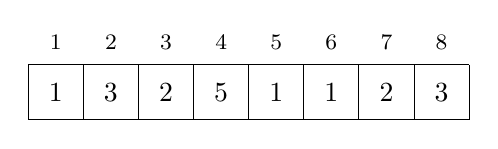
\begin{tikzpicture}[scale=0.7]
\draw (0,0) grid (8,1);

\node at (0.5,0.5) {$1$};
\node at (1.5,0.5) {$3$};
\node at (2.5,0.5) {$2$};
\node at (3.5,0.5) {$5$};
\node at (4.5,0.5) {$1$};
\node at (5.5,0.5) {$1$};
\node at (6.5,0.5) {$2$};
\node at (7.5,0.5) {$3$};

\footnotesize
\node at (0.5,1.4) {$1$};
\node at (1.5,1.4) {$2$};
\node at (2.5,1.4) {$3$};
\node at (3.5,1.4) {$4$};
\node at (4.5,1.4) {$5$};
\node at (5.5,1.4) {$6$};
\node at (6.5,1.4) {$7$};
\node at (7.5,1.4) {$8$};
\end{tikzpicture}
\end{center}
contains a subarray with sum 8:
\begin{center}
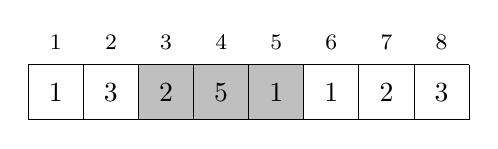
\begin{tikzpicture}[scale=0.7]
\fill[color=lightgray] (2,0) rectangle (5,1);
\draw (0,0) grid (8,1);

\node at (0.5,0.5) {$1$};
\node at (1.5,0.5) {$3$};
\node at (2.5,0.5) {$2$};
\node at (3.5,0.5) {$5$};
\node at (4.5,0.5) {$1$};
\node at (5.5,0.5) {$1$};
\node at (6.5,0.5) {$2$};
\node at (7.5,0.5) {$3$};

\footnotesize
\node at (0.5,1.4) {$1$};
\node at (1.5,1.4) {$2$};
\node at (2.5,1.4) {$3$};
\node at (3.5,1.4) {$4$};
\node at (4.5,1.4) {$5$};
\node at (5.5,1.4) {$6$};
\node at (6.5,1.4) {$7$};
\node at (7.5,1.4) {$8$};
\end{tikzpicture}
\end{center}

It turns out that the problem can be solved in
$O(n)$ time using the two pointers method.
The idea is to iterate through the array
using two pointers that define a range in the array.
On each turn, the left pointer moves one step
forward, and the right pointer moves forward
as long as the sum is at most $x$.
If the sum of the range becomes exactly $x$,
we have found a solution.

As an example, we consider the following array
with target sum $x=8$:
\begin{center}
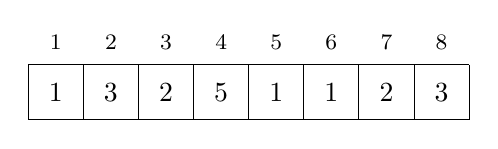
\begin{tikzpicture}[scale=0.7]
\draw (0,0) grid (8,1);

\node at (0.5,0.5) {$1$};
\node at (1.5,0.5) {$3$};
\node at (2.5,0.5) {$2$};
\node at (3.5,0.5) {$5$};
\node at (4.5,0.5) {$1$};
\node at (5.5,0.5) {$1$};
\node at (6.5,0.5) {$2$};
\node at (7.5,0.5) {$3$};

\footnotesize
\node at (0.5,1.4) {$1$};
\node at (1.5,1.4) {$2$};
\node at (2.5,1.4) {$3$};
\node at (3.5,1.4) {$4$};
\node at (4.5,1.4) {$5$};
\node at (5.5,1.4) {$6$};
\node at (6.5,1.4) {$7$};
\node at (7.5,1.4) {$8$};
\end{tikzpicture}
\end{center}

First, the pointers define a range with sum $1+3+2=6$.
The range can't be larger
because the next number 5 would make the sum
larger than $x$.

\begin{center}
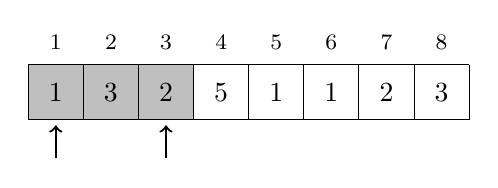
\begin{tikzpicture}[scale=0.7]
\fill[color=lightgray] (0,0) rectangle (3,1);
\draw (0,0) grid (8,1);

\node at (0.5,0.5) {$1$};
\node at (1.5,0.5) {$3$};
\node at (2.5,0.5) {$2$};
\node at (3.5,0.5) {$5$};
\node at (4.5,0.5) {$1$};
\node at (5.5,0.5) {$1$};
\node at (6.5,0.5) {$2$};
\node at (7.5,0.5) {$3$};

\draw[thick,->] (0.5,-0.7) -- (0.5,-0.1);
\draw[thick,->] (2.5,-0.7) -- (2.5,-0.1);

\footnotesize
\node at (0.5,1.4) {$1$};
\node at (1.5,1.4) {$2$};
\node at (2.5,1.4) {$3$};
\node at (3.5,1.4) {$4$};
\node at (4.5,1.4) {$5$};
\node at (5.5,1.4) {$6$};
\node at (6.5,1.4) {$7$};
\node at (7.5,1.4) {$8$};
\end{tikzpicture}
\end{center}

After this, the left pointer moves one step forward.
The right pointer doesn't move because otherwise
the sum would become too large.

\begin{center}
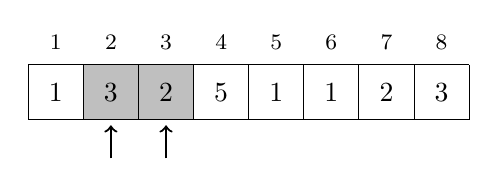
\begin{tikzpicture}[scale=0.7]
\fill[color=lightgray] (1,0) rectangle (3,1);
\draw (0,0) grid (8,1);

\node at (0.5,0.5) {$1$};
\node at (1.5,0.5) {$3$};
\node at (2.5,0.5) {$2$};
\node at (3.5,0.5) {$5$};
\node at (4.5,0.5) {$1$};
\node at (5.5,0.5) {$1$};
\node at (6.5,0.5) {$2$};
\node at (7.5,0.5) {$3$};

\draw[thick,->] (1.5,-0.7) -- (1.5,-0.1);
\draw[thick,->] (2.5,-0.7) -- (2.5,-0.1);

\footnotesize
\node at (0.5,1.4) {$1$};
\node at (1.5,1.4) {$2$};
\node at (2.5,1.4) {$3$};
\node at (3.5,1.4) {$4$};
\node at (4.5,1.4) {$5$};
\node at (5.5,1.4) {$6$};
\node at (6.5,1.4) {$7$};
\node at (7.5,1.4) {$8$};
\end{tikzpicture}
\end{center}

Again, the left pointer moves one step forward,
and this time the right pointer moves three
steps forward.
The sum is $2+5+1=8$, so we have found a subarray
where the sum of the elements is $x$.

\begin{center}
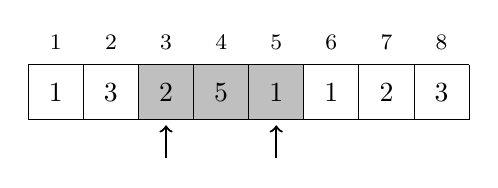
\begin{tikzpicture}[scale=0.7]
\fill[color=lightgray] (2,0) rectangle (5,1);
\draw (0,0) grid (8,1);

\node at (0.5,0.5) {$1$};
\node at (1.5,0.5) {$3$};
\node at (2.5,0.5) {$2$};
\node at (3.5,0.5) {$5$};
\node at (4.5,0.5) {$1$};
\node at (5.5,0.5) {$1$};
\node at (6.5,0.5) {$2$};
\node at (7.5,0.5) {$3$};

\draw[thick,->] (2.5,-0.7) -- (2.5,-0.1);
\draw[thick,->] (4.5,-0.7) -- (4.5,-0.1);

\footnotesize
\node at (0.5,1.4) {$1$};
\node at (1.5,1.4) {$2$};
\node at (2.5,1.4) {$3$};
\node at (3.5,1.4) {$4$};
\node at (4.5,1.4) {$5$};
\node at (5.5,1.4) {$6$};
\node at (6.5,1.4) {$7$};
\node at (7.5,1.4) {$8$};
\end{tikzpicture}
\end{center}

The time complexity of the algorithm depends on
the number of steps the right pointer moves.
There is no upper bound how many steps the
pointer can move on a single turn.
However, the pointer moves \emph{a total of}
$O(n)$ steps during the algorithm
because it only moves forward.

Since both the left and the right pointer
move $O(n)$ steps during the algorithm,
the time complexity is $O(n)$.

\subsubsection{Sum of two numbers}

\index{2SUM problem}

Given an array of $n$ integers and an integer $x$,
our task is to find two numbers in array
whose sum is $x$ or report that there are no such numbers.
This problem is known as the \key{2SUM} problem,
and it can be solved efficiently using the
two pointers method.

First, we sort the numbers in the array in
increasing order.
After this, we iterate through the array using
two pointers that begin at both ends of the array.
The left pointer begins from the first element
and moves one step forward on each turn.
The right pointer begins from the last element
and always moves backward until the sum of the range
defined by the pointers is at most $x$.
If the sum is exactly $x$, we have found a solution.

For example, consider the following array when
our task is to find two elements whose sum is $x=12$:
\begin{center}
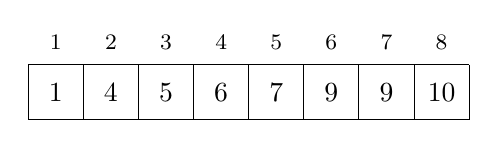
\begin{tikzpicture}[scale=0.7]
\draw (0,0) grid (8,1);

\node at (0.5,0.5) {$1$};
\node at (1.5,0.5) {$4$};
\node at (2.5,0.5) {$5$};
\node at (3.5,0.5) {$6$};
\node at (4.5,0.5) {$7$};
\node at (5.5,0.5) {$9$};
\node at (6.5,0.5) {$9$};
\node at (7.5,0.5) {$10$};

\footnotesize
\node at (0.5,1.4) {$1$};
\node at (1.5,1.4) {$2$};
\node at (2.5,1.4) {$3$};
\node at (3.5,1.4) {$4$};
\node at (4.5,1.4) {$5$};
\node at (5.5,1.4) {$6$};
\node at (6.5,1.4) {$7$};
\node at (7.5,1.4) {$8$};
\end{tikzpicture}
\end{center}

The initial positions of the pointers
are as follows.
The sum of the numbers is $1+10=11$
that is smaller than $x$.

\begin{center}
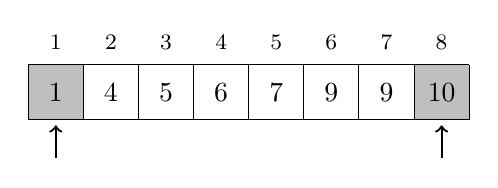
\begin{tikzpicture}[scale=0.7]
\fill[color=lightgray] (0,0) rectangle (1,1);
\fill[color=lightgray] (7,0) rectangle (8,1);
\draw (0,0) grid (8,1);

\node at (0.5,0.5) {$1$};
\node at (1.5,0.5) {$4$};
\node at (2.5,0.5) {$5$};
\node at (3.5,0.5) {$6$};
\node at (4.5,0.5) {$7$};
\node at (5.5,0.5) {$9$};
\node at (6.5,0.5) {$9$};
\node at (7.5,0.5) {$10$};

\draw[thick,->] (0.5,-0.7) -- (0.5,-0.1);
\draw[thick,->] (7.5,-0.7) -- (7.5,-0.1);

\footnotesize
\node at (0.5,1.4) {$1$};
\node at (1.5,1.4) {$2$};
\node at (2.5,1.4) {$3$};
\node at (3.5,1.4) {$4$};
\node at (4.5,1.4) {$5$};
\node at (5.5,1.4) {$6$};
\node at (6.5,1.4) {$7$};
\node at (7.5,1.4) {$8$};
\end{tikzpicture}
\end{center}

Then the left pointer moves one step forward.
The right pointer moves three steps backward,
and the sum becomes $4+7=11$.

\begin{center}
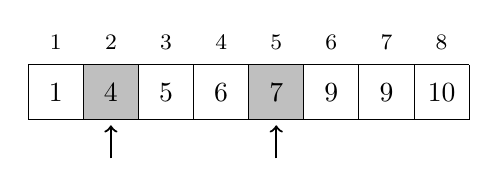
\begin{tikzpicture}[scale=0.7]
\fill[color=lightgray] (1,0) rectangle (2,1);
\fill[color=lightgray] (4,0) rectangle (5,1);
\draw (0,0) grid (8,1);

\node at (0.5,0.5) {$1$};
\node at (1.5,0.5) {$4$};
\node at (2.5,0.5) {$5$};
\node at (3.5,0.5) {$6$};
\node at (4.5,0.5) {$7$};
\node at (5.5,0.5) {$9$};
\node at (6.5,0.5) {$9$};
\node at (7.5,0.5) {$10$};

\draw[thick,->] (1.5,-0.7) -- (1.5,-0.1);
\draw[thick,->] (4.5,-0.7) -- (4.5,-0.1);

\footnotesize
\node at (0.5,1.4) {$1$};
\node at (1.5,1.4) {$2$};
\node at (2.5,1.4) {$3$};
\node at (3.5,1.4) {$4$};
\node at (4.5,1.4) {$5$};
\node at (5.5,1.4) {$6$};
\node at (6.5,1.4) {$7$};
\node at (7.5,1.4) {$8$};
\end{tikzpicture}
\end{center}

After this, the left pointer moves one step forward again.
The right pointer doesn't move, and the solution
$5+7=12$ has been found.

\begin{center}
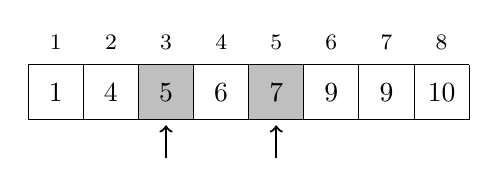
\begin{tikzpicture}[scale=0.7]
\fill[color=lightgray] (2,0) rectangle (3,1);
\fill[color=lightgray] (4,0) rectangle (5,1);
\draw (0,0) grid (8,1);

\node at (0.5,0.5) {$1$};
\node at (1.5,0.5) {$4$};
\node at (2.5,0.5) {$5$};
\node at (3.5,0.5) {$6$};
\node at (4.5,0.5) {$7$};
\node at (5.5,0.5) {$9$};
\node at (6.5,0.5) {$9$};
\node at (7.5,0.5) {$10$};

\draw[thick,->] (2.5,-0.7) -- (2.5,-0.1);
\draw[thick,->] (4.5,-0.7) -- (4.5,-0.1);

\footnotesize
\node at (0.5,1.4) {$1$};
\node at (1.5,1.4) {$2$};
\node at (2.5,1.4) {$3$};
\node at (3.5,1.4) {$4$};
\node at (4.5,1.4) {$5$};
\node at (5.5,1.4) {$6$};
\node at (6.5,1.4) {$7$};
\node at (7.5,1.4) {$8$};
\end{tikzpicture}
\end{center}

At the beginning of the algorithm,
the sorting takes $O(n \log n)$ time.
After this, the left pointer moves $O(n)$ steps
forward, and the right pointer moves $O(n)$ steps
backward. Thus, the total time complexity
of the algorithm is $O(n \log n)$.

Note that it is possible to solve
in another way in $O(n \log n)$ time using binary search.
In this solution, we iterate through the array
and for each number, we try to find another
number such that the sum is $x$.
This can be done by performing $n$ binary searches,
and each search takes $O(\log n)$ time.

\index{3SUM-ongelma}
A somewhat more difficult problem is 
the \key{3SUM} problem where our task is
to find \emph{three} numbers whose sum is $x$.
This problem can be solved in $O(n^2)$ time.
Can you see how it is possible?

\section{Nearest smaller elements}

\index{nearest smaller elements}

Amortized analysis is often used for
estimating the number of operations
performed for a data structure.
The operations may be distributed unevenly so
that the most operations appear during a
certain phase in the algorithm, but the total
number of the operations is limited.

As an example, let us consider a problem
where our task is to find for each element
in an array the
\key{nearest smaller element}, i.e.,
the nearest smaller element that precedes
the element in the array.
It is possible that no such element exists,
and the algorithm should notice this.
It turns out that the problem can be efficiently solved
in $O(n)$ time using a suitable data structure.

An efficient solution for the problem is to
iterate through the array from the left to the right,
and maintain a chain of elements where the
first element is the active element in the array
and each following element is the nearest smaller
element of the previous element.
If the chain only contains one element,
the active element doesn't have a nearest smaller element.
At each step, we remove elements from the chain
until the first element is smaller
than the active element, or the chain is empty.
After this, the active element becomes the first element
in the chain.

As an example, consider the following array:
\begin{center}
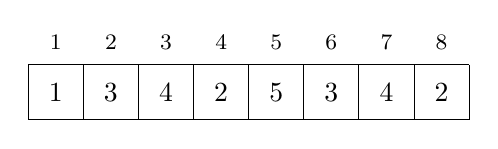
\begin{tikzpicture}[scale=0.7]
\draw (0,0) grid (8,1);

\node at (0.5,0.5) {$1$};
\node at (1.5,0.5) {$3$};
\node at (2.5,0.5) {$4$};
\node at (3.5,0.5) {$2$};
\node at (4.5,0.5) {$5$};
\node at (5.5,0.5) {$3$};
\node at (6.5,0.5) {$4$};
\node at (7.5,0.5) {$2$};

\footnotesize
\node at (0.5,1.4) {$1$};
\node at (1.5,1.4) {$2$};
\node at (2.5,1.4) {$3$};
\node at (3.5,1.4) {$4$};
\node at (4.5,1.4) {$5$};
\node at (5.5,1.4) {$6$};
\node at (6.5,1.4) {$7$};
\node at (7.5,1.4) {$8$};
\end{tikzpicture}
\end{center}

First, numbers 1, 3 and 4 are added to the chain
because each element is larger than the previous element.
This means that the nearest smaller element of
number 4 is number 3 whose nearest smaller element
is number 1.
\begin{center}
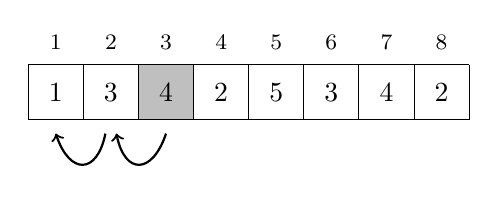
\begin{tikzpicture}[scale=0.7]
\fill[color=lightgray] (2,0) rectangle (3,1);
\draw (0,0) grid (8,1);

\node at (0.5,0.5) {$1$};
\node at (1.5,0.5) {$3$};
\node at (2.5,0.5) {$4$};
\node at (3.5,0.5) {$2$};
\node at (4.5,0.5) {$5$};
\node at (5.5,0.5) {$3$};
\node at (6.5,0.5) {$4$};
\node at (7.5,0.5) {$2$};

\draw[thick,->] (2.5,-0.25) .. controls (2.25,-1.00) and (1.75,-1.00) .. (1.6,-0.25);
\draw[thick,->] (1.4,-0.25) .. controls (1.25,-1.00) and (0.75,-1.00) .. (0.5,-0.25);

\footnotesize
\node at (0.5,1.4) {$1$};
\node at (1.5,1.4) {$2$};
\node at (2.5,1.4) {$3$};
\node at (3.5,1.4) {$4$};
\node at (4.5,1.4) {$5$};
\node at (5.5,1.4) {$6$};
\node at (6.5,1.4) {$7$};
\node at (7.5,1.4) {$8$};
\end{tikzpicture}
\end{center}

The next number 2 is smaller than two first numbers in the chain.
Thus, numbers 4 and 3 are removed, and then number 2 becomes
the first element in the chain.
Its nearest smaller element is number 1:
\begin{center}
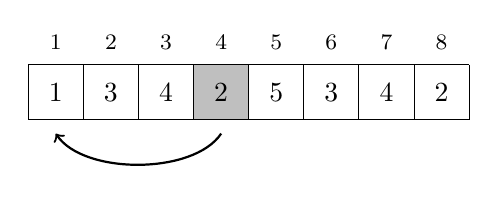
\begin{tikzpicture}[scale=0.7]
\fill[color=lightgray] (3,0) rectangle (4,1);
\draw (0,0) grid (8,1);

\node at (0.5,0.5) {$1$};
\node at (1.5,0.5) {$3$};
\node at (2.5,0.5) {$4$};
\node at (3.5,0.5) {$2$};
\node at (4.5,0.5) {$5$};
\node at (5.5,0.5) {$3$};
\node at (6.5,0.5) {$4$};
\node at (7.5,0.5) {$2$};

\draw[thick,->] (3.5,-0.25) .. controls (3.00,-1.00) and (1.00,-1.00) .. (0.5,-0.25);

\footnotesize
\node at (0.5,1.4) {$1$};
\node at (1.5,1.4) {$2$};
\node at (2.5,1.4) {$3$};
\node at (3.5,1.4) {$4$};
\node at (4.5,1.4) {$5$};
\node at (5.5,1.4) {$6$};
\node at (6.5,1.4) {$7$};
\node at (7.5,1.4) {$8$};
\end{tikzpicture}
\end{center}

After this, number 5 is larger than number 2,
so it will be added to the chain and
its nearest smaller element is number 2:
\begin{center}
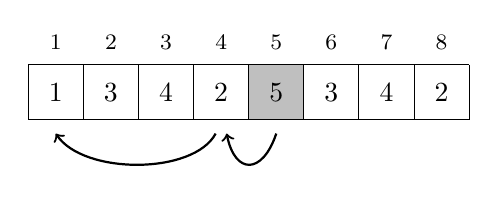
\begin{tikzpicture}[scale=0.7]
\fill[color=lightgray] (4,0) rectangle (5,1);
\draw (0,0) grid (8,1);

\node at (0.5,0.5) {$1$};
\node at (1.5,0.5) {$3$};
\node at (2.5,0.5) {$4$};
\node at (3.5,0.5) {$2$};
\node at (4.5,0.5) {$5$};
\node at (5.5,0.5) {$3$};
\node at (6.5,0.5) {$4$};
\node at (7.5,0.5) {$2$};

\draw[thick,->] (3.4,-0.25) .. controls (3.00,-1.00) and (1.00,-1.00) .. (0.5,-0.25);
\draw[thick,->] (4.5,-0.25) .. controls (4.25,-1.00) and (3.75,-1.00) .. (3.6,-0.25);

\footnotesize
\node at (0.5,1.4) {$1$};
\node at (1.5,1.4) {$2$};
\node at (2.5,1.4) {$3$};
\node at (3.5,1.4) {$4$};
\node at (4.5,1.4) {$5$};
\node at (5.5,1.4) {$6$};
\node at (6.5,1.4) {$7$};
\node at (7.5,1.4) {$8$};
\end{tikzpicture}
\end{center}

Algorithm continues in a similar way
and finds out the nearest smaller element
for each number in the array.
But how efficient is the algorithm?

The efficiency of the algorithm depends on
the total time used for manipulating the chain.
If an element is larger than the first
element in the chain, it will only be inserted
to the beginning of the chain which is efficient.
However, sometimes the chain can contain several
larger elements and it takes time to remove them.
Still, each element is added exactly once to the chain
and removed at most once.
Thus, each element causes $O(1)$ operations
to the chain, and the total time complexity
of the algorithm is $O(n)$.

\section{Liukuvan ikkunan minimi}

\index{liukuva ikkuna}
\index{liukuvan ikkunan minimi@liukuvan ikkunan minimi}

\key{Liukuva ikkuna} on taulukon halki kulkeva
aktiivinen alitaulukko, jonka pituus on vakio.
Jokaisessa liukuvan ikkunan sijainnissa
halutaan tyypillisesti laskea jotain tietoa
ikkunan alueelle osuvista alkioista.
Kiinnostava tehtävä on pitää yllä
\key{liukuvan ikkunan minimiä}.
Tämä tarkoittaa, että jokaisessa liukuvan ikkunan
sijainnissa tulee ilmoittaa pienin alkio
ikkunan alueella.

Liukuvan ikkunan minimit voi laskea
lähes samalla tavalla kuin lähimmät
pienimmät edeltäjät.
Ideana on pitää yllä ketjua, jonka alussa
on ikkunan viimeinen luku ja jossa jokainen
luku on edellistä pienempi. Joka vaiheessa
ketjun viimeinen luku on ikkunan pienin luku.
Kun liukuva ikkuna liikkuu eteenpäin ja välille
tulee uusi luku, ketjusta poistetaan kaikki luvut,
jotka ovat uutta lukua suurempia.
Tämän jälkeen uusi luku lisätään ketjun alkuun.
Lisäksi jos ketjun viimeinen luku ei enää kuulu
välille, se poistetaan ketjusta.

Tarkastellaan esimerkkinä, kuinka algoritmi selvittää
minimit seuraavassa taulukossa,
kun ikkunan koko $k=4$.

\begin{center}
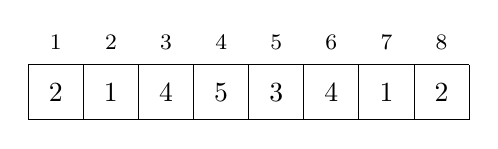
\begin{tikzpicture}[scale=0.7]
\draw (0,0) grid (8,1);

\node at (0.5,0.5) {$2$};
\node at (1.5,0.5) {$1$};
\node at (2.5,0.5) {$4$};
\node at (3.5,0.5) {$5$};
\node at (4.5,0.5) {$3$};
\node at (5.5,0.5) {$4$};
\node at (6.5,0.5) {$1$};
\node at (7.5,0.5) {$2$};

\footnotesize
\node at (0.5,1.4) {$1$};
\node at (1.5,1.4) {$2$};
\node at (2.5,1.4) {$3$};
\node at (3.5,1.4) {$4$};
\node at (4.5,1.4) {$5$};
\node at (5.5,1.4) {$6$};
\node at (6.5,1.4) {$7$};
\node at (7.5,1.4) {$8$};
\end{tikzpicture}
\end{center}

Liukuva ikkuna aloittaa matkansa taulukon vasemmasta reunasta.
Ensimmäisessä ikkunan sijainnissa pienin luku on 1:
\begin{center}
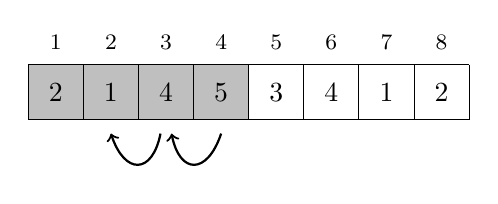
\begin{tikzpicture}[scale=0.7]
\fill[color=lightgray] (0,0) rectangle (4,1);
\draw (0,0) grid (8,1);

\node at (0.5,0.5) {$2$};
\node at (1.5,0.5) {$1$};
\node at (2.5,0.5) {$4$};
\node at (3.5,0.5) {$5$};
\node at (4.5,0.5) {$3$};
\node at (5.5,0.5) {$4$};
\node at (6.5,0.5) {$1$};
\node at (7.5,0.5) {$2$};

\footnotesize
\node at (0.5,1.4) {$1$};
\node at (1.5,1.4) {$2$};
\node at (2.5,1.4) {$3$};
\node at (3.5,1.4) {$4$};
\node at (4.5,1.4) {$5$};
\node at (5.5,1.4) {$6$};
\node at (6.5,1.4) {$7$};
\node at (7.5,1.4) {$8$};

\draw[thick,->] (3.5,-0.25) .. controls (3.25,-1.00) and (2.75,-1.00) .. (2.6,-0.25);
\draw[thick,->] (2.4,-0.25) .. controls (2.25,-1.00) and (1.75,-1.00) .. (1.5,-0.25);

\end{tikzpicture}
\end{center}

Kun ikkuna siirtyy eteenpäin, mukaan tulee luku 3,
joka on pienempi kuin luvut 5 ja 4 ketjun alussa.
Niinpä luvut 5 ja 4 poistuvat ketjusta ja luku 3
siirtyy sen alkuun. Pienin luku on edelleen 1.
\begin{center}
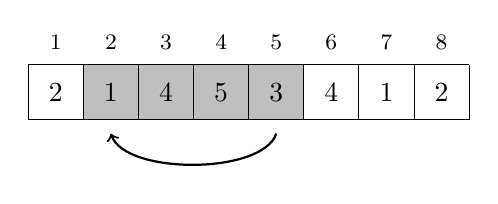
\begin{tikzpicture}[scale=0.7]
\fill[color=lightgray] (1,0) rectangle (5,1);
\draw (0,0) grid (8,1);

\node at (0.5,0.5) {$2$};
\node at (1.5,0.5) {$1$};
\node at (2.5,0.5) {$4$};
\node at (3.5,0.5) {$5$};
\node at (4.5,0.5) {$3$};
\node at (5.5,0.5) {$4$};
\node at (6.5,0.5) {$1$};
\node at (7.5,0.5) {$2$};

\footnotesize
\node at (0.5,1.4) {$1$};
\node at (1.5,1.4) {$2$};
\node at (2.5,1.4) {$3$};
\node at (3.5,1.4) {$4$};
\node at (4.5,1.4) {$5$};
\node at (5.5,1.4) {$6$};
\node at (6.5,1.4) {$7$};
\node at (7.5,1.4) {$8$};

\draw[thick,->] (4.5,-0.25) .. controls (4.25,-1.00) and (1.75,-1.00) .. (1.5,-0.25);

\end{tikzpicture}
\end{center}

Ikkuna siirtyy taas eteenpäin, minkä seurauksena pienin luku 1
putoaa pois ikkunasta. Niinpä se poistetaan ketjun lopusta
ja uusi pienin luku on 3. Lisäksi uusi ikkunaan tuleva luku 4
lisätään ketjun alkuun.
\begin{center}
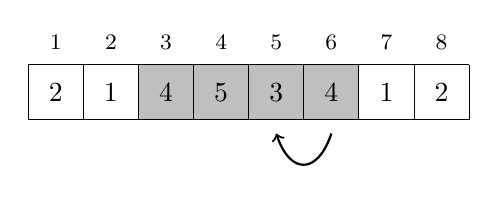
\begin{tikzpicture}[scale=0.7]
\fill[color=lightgray] (2,0) rectangle (6,1);
\draw (0,0) grid (8,1);

\node at (0.5,0.5) {$2$};
\node at (1.5,0.5) {$1$};
\node at (2.5,0.5) {$4$};
\node at (3.5,0.5) {$5$};
\node at (4.5,0.5) {$3$};
\node at (5.5,0.5) {$4$};
\node at (6.5,0.5) {$1$};
\node at (7.5,0.5) {$2$};

\footnotesize
\node at (0.5,1.4) {$1$};
\node at (1.5,1.4) {$2$};
\node at (2.5,1.4) {$3$};
\node at (3.5,1.4) {$4$};
\node at (4.5,1.4) {$5$};
\node at (5.5,1.4) {$6$};
\node at (6.5,1.4) {$7$};
\node at (7.5,1.4) {$8$};

\draw[thick,->] (5.5,-0.25) .. controls (5.25,-1.00) and (4.75,-1.00) .. (4.5,-0.25);
\end{tikzpicture}
\end{center}

Seuraavaksi ikkunaan tuleva luku 1 on pienempi
kuin kaikki ketjussa olevat luvut.
Tämän seurauksena koko ketju tyhjentyy ja
siihen jää vain luku 1:
\begin{center}
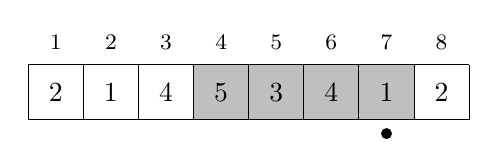
\begin{tikzpicture}[scale=0.7]
\fill[color=lightgray] (3,0) rectangle (7,1);
\draw (0,0) grid (8,1);

\node at (0.5,0.5) {$2$};
\node at (1.5,0.5) {$1$};
\node at (2.5,0.5) {$4$};
\node at (3.5,0.5) {$5$};
\node at (4.5,0.5) {$3$};
\node at (5.5,0.5) {$4$};
\node at (6.5,0.5) {$1$};
\node at (7.5,0.5) {$2$};

\footnotesize
\node at (0.5,1.4) {$1$};
\node at (1.5,1.4) {$2$};
\node at (2.5,1.4) {$3$};
\node at (3.5,1.4) {$4$};
\node at (4.5,1.4) {$5$};
\node at (5.5,1.4) {$6$};
\node at (6.5,1.4) {$7$};
\node at (7.5,1.4) {$8$};

\fill[color=black] (6.5,-0.25) circle (0.1);

%\draw[thick,->] (5.5,-0.25) .. controls (5.25,-1.00) and (4.75,-1.00) .. (4.5,-0.25);
\end{tikzpicture}
\end{center}

Lopuksi ikkuna saapuu viimeiseen sijaintiinsa.
Luku 2 lisätään ketjun alkuun,
mutta ikkunan pienin luku on edelleen 1.
\begin{center}
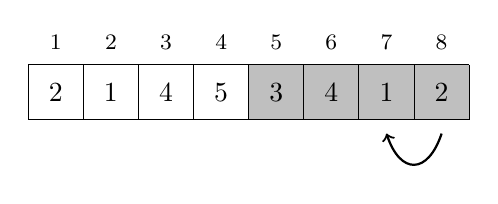
\begin{tikzpicture}[scale=0.7]
\fill[color=lightgray] (4,0) rectangle (8,1);
\draw (0,0) grid (8,1);

\node at (0.5,0.5) {$2$};
\node at (1.5,0.5) {$1$};
\node at (2.5,0.5) {$4$};
\node at (3.5,0.5) {$5$};
\node at (4.5,0.5) {$3$};
\node at (5.5,0.5) {$4$};
\node at (6.5,0.5) {$1$};
\node at (7.5,0.5) {$2$};

\footnotesize
\node at (0.5,1.4) {$1$};
\node at (1.5,1.4) {$2$};
\node at (2.5,1.4) {$3$};
\node at (3.5,1.4) {$4$};
\node at (4.5,1.4) {$5$};
\node at (5.5,1.4) {$6$};
\node at (6.5,1.4) {$7$};
\node at (7.5,1.4) {$8$};

\draw[thick,->] (7.5,-0.25) .. controls (7.25,-1.00) and (6.75,-1.00) .. (6.5,-0.25);
\end{tikzpicture}
\end{center}

Tässäkin algoritmissa jokainen taulukon luku lisätään
ketjuun tarkalleen kerran ja poistetaan ketjusta korkeintaan kerran,
joko ketjun alusta tai ketjun lopusta.
Niinpä algoritmin kokonaisaikavaativuus on $O(n)$.



